\documentclass[tikz,border=2pt]{standalone}
\usepackage{amsmath,amssymb}
\usepackage{pgfplots}
\pgfplotsset{compat=1.18}

\begin{document}
% The standard normal density phi(z) with mean 0 and variance 1; the shaded area up to z = 1
% is Phi(1) = 0.8413, the value tabulated in the standard normal table.
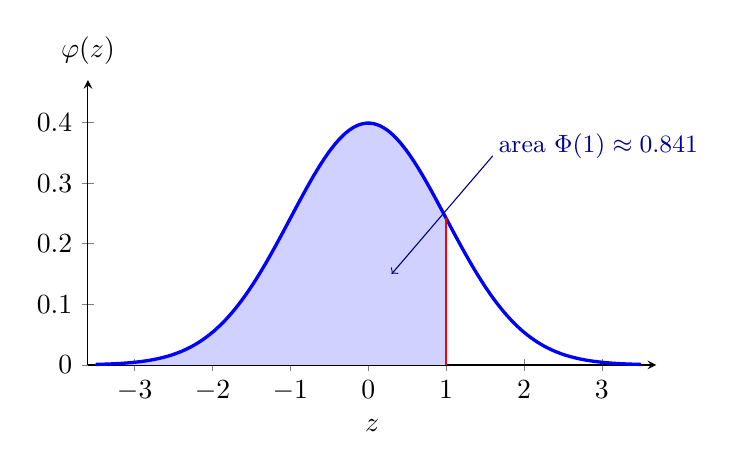
\begin{tikzpicture}
	\begin{axis}[
		axis lines=left, xmin=-3.6, xmax=3.7, ymin=0, ymax=0.47,
		xtick={-3,-2,-1,0,1,2,3}, ytick={0,0.1,0.2,0.3,0.4},
		xlabel={$z$}, ylabel={$\varphi(z)$}, ylabel style={rotate=-90, anchor=south, at={(axis description cs:0,1.02)}},
		samples=160, smooth, width=8.8cm, height=5.2cm, clip=false
		]
		\addplot[fill=blue!18, draw=none, domain=-3.5:1] {exp(-x^2/2)/sqrt(2*pi)} \closedcycle;
		\addplot[blue, very thick, domain=-3.5:3.5] {exp(-x^2/2)/sqrt(2*pi)};
		\draw[red, thick] (axis cs:1,0) -- (axis cs:1,0.242);
		\node[blue!60!black, font=\small, anchor=west] at (axis cs:1.55,0.36) {area $\Phi(1)\approx0.841$};
		\draw[blue!60!black, ->] (axis cs:1.6,0.345) -- (axis cs:0.3,0.15);
	\end{axis}
	
\end{tikzpicture}
\end{document}
